\documentclass[professionalfont]{beamer}
\usepackage{newtxtext}
\usepackage[heading = false, scheme = plain]{ctex}
\mode<presentation>{\usetheme{Warsaw}}
%\usecolortheme{dove}
\setbeamertemplate{footline}{}
\beamertemplatenavigationsymbolsempty
\addtobeamertemplate{navigation symbols}{}{%
    \usebeamerfont{footline}%
    \usebeamercolor[black]{footline}%
    \hspace{1em}%
    \insertframenumber/\inserttotalframenumber
}
\setbeamertemplate{caption}[numbered]
\usepackage{hyperref} 
\usepackage{bbm}
\usepackage{multirow}
\usepackage{amsmath}
\usepackage{listings}
\usepackage{natbib}
\usepackage{xcolor}
\lstset{basicstyle=\tiny\ttfamily,
	numbers=left,
	escapeinside=||
}
\newcommand{\R}[1]{\textcolor{blue}{\small \textrm{#1}}}
\newcommand{\Rout}[1]{\textcolor{green}{\small \textrm{#1}}}
\newcommand{\red}[1]{\textcolor{red}{#1}}
\newcommand{\green}[1]{\textbf{#1}}
\newcommand{\purple}[1]{\textcolor{purple}{#1}}
\newcommand{\blue}[1]{\textcolor{blue}{#1}}
\newcommand{\gray}[1]{\textcolor{gray}{#1}}

\title{第3讲:费率厘定基础~2}
\author{高光远}
\institute{中国人民大学~统计学院}
\date{}
\begin{document}
%%title frame
\begin{frame}
	\titlepage
\end{frame}

\begin{frame}{主要内容}
	\tableofcontents
\end{frame}

%%table of contents
%\AtBeginSection[]
%{
%	\begin{frame}{}
%		\tableofcontents[currentsection]
%	\end{frame}
%}


%%normal frame
\section{数据的类型}
	\begin{frame}
	\begin{itemize}
		\item 风险信息:~风险单位数, 保费, 索赔次数, 索赔金额, 风险因子, 直接理赔费用等.
		\item 会计信息: 承保费用, 间接理赔费用等. 
		\item 风险信息中有两类数据: 
		\begin{enumerate}
			\item \red{保单数据库(policy database)}
			\item \red{索赔数据库(claim database)}
			\end{enumerate}
		\end{itemize}	
	\end{frame}
		
\subsection{保单数据库}
\begin{frame}
	假设三份保单的交易情况如下:
\begin{enumerate}
	\item[A:]生效日期是2011年1月1日, 年保费是900元, 免赔额是500元.
	\item[B:]生效日期是2011年4月1日, 年保费是800元, 免赔额是500元. 该保单在2011年12月31日\green{撤销}。
	\item[C:]生效日期是2011年7月1日, 年保费是900元, 免赔额是700元. 在2012年1月1日, \green{被保险人将免赔额降低为500元}, 降低免赔额后的年保费为1000元。
\end{enumerate}
{\scriptsize \begin{table}[]
	\centering
	\caption{风险单位数和保费的记录}
	\label{my-label}
	\begin{tabular}{ccccccc}
		\hline
		保单 & \multirow{2}{*}{生效日} & \multirow{2}{*}{到期日} & \multirow{2}{*}{交易日} & \multirow{2}{*}{免赔额} & 承保风险  & 承保   \\
		编码 &                      &                      &                      &                      & 单位数   & 保费   \\ \hline
		A  & \green{2011.1.1}             & 2011.12.31           & \green{2010.12.15}           & 500                  & 1     & 900  \\
		B  & 2011.4.1             & 2012.3.31            & 2011.4.1             & 500                  & 1     & 800  \\
		B  & 2011.4.1             & 2012.3.31            & 2011.12.31           & 500                  & -0.25 & -200 \\
		C  & \green{2011.7.1}             & 2012.6.30            & \green{2011.6.20}            & 700                  & 1     & 900  \\
		C  & 2011.7.1             & 2012.6.30            & 2012.1.1             & 700                  & -0.5  & -450 \\
		C  & 2011.7.1             & 2012.6.30            & 2012.1.1             & 500                  & 0.5   & 500  \\ \hline
	\end{tabular}
\end{table}}
\end{frame}
\begin{frame}{}
	\begin{itemize}
		\item 如何记录由于中途退保或保额改变而造成的保费变动?\\
		原则: 原有记录保持不变, 增加新的记录.
		\item 注意: 发生承保的交易日也称为\green{承保日期}, 但可能和\green{生效日期}不同. 
		\item 有时承保日期和生效日期混用, 需要具体问题具体分析. 
		\item 通常, ``字段说明''文件会详细解释各字段的意义.
	\end{itemize}
\end{frame}
\begin{frame}{实例}
某保险公司提供的保单数据库\href{https://www.jianguoyun.com/p/DcrJkekQyKLGBhjEsUU}{(点击可下载)}包含以下二十个字段:
		
		~
		
		\begin{enumerate}
			\item \blue{保单编码(POLICYCODE)}: 有\green{12076}份保单.
			\item \blue{地区(BRANCHNAME)}: 保单分布于\green{27}个省份.
			\item \blue{险种(RISKCODE)}: \green{6049}份交强险; \green{6027}份商业险.  
			\item \blue{险别(KINDCODE)}: 交强险只有\green{一}种类型. 商业险可包含\green{七}种类型: 三者险, 车损险, 驾驶员保险, 乘客保险, 玻璃破碎险, 盗抢险, 和划痕险.
		\item 承保时间(UNDERWRITTENDATE): 从 \green{2013-10-19} 到 \green{2017-06-30}.
		\item \blue{生效日(KINDSTARTDATE)}: 从 \green{2014-01-01} 到 \green{2017-09-25}.
		\item \blue{到期日(DUEENDDATE)}: 从 \green{2014-03-22} 到 \green{2018-09-24}.
		\end{enumerate}
	\end{frame}
\begin{frame}{实例}	
\begin{enumerate}	
	\setcounter{enumi}{7}

\item 新车购置价(PURCHASEPRICENOTAX): 从\green{25,000}到\green{990,000} CNY.
\item 座位数(SEATCOUNT): 从\green{2}个到\green{8}个.
\item 品牌(CARBRAND): \green{67}种.
\item 车系(CARSERIESNAME): \green{285}个系列.
\item \blue{年龄(AGE)}:  从\green{18}岁到\green{77}岁.
\item \blue{性别(SEX)}: 1代表男性(\green{8397}份), 2代表女性(\green{3674}份). 
\item \blue{车龄(USEYEARS)}: 从\green{0}年到\green{14}年.
\end{enumerate}

~

8主要用于车损险的费率厘定中; 12-14为常用的风险因子.
\end{frame}

\begin{frame}{实例}	
	\begin{enumerate}	
		\setcounter{enumi}{14}
		\item 无赔款优待系数(WPRATE0506): 商业险NCD(no claim discount), 从0.5到1.5.
		\item 无赔款优待系数(WPRATE0507): 交强险NCD(no claim discount), 从0.7到1.3.
		\item 上年出险次数(LASTCLAIMCOUNT): -3为新车, -4为新保, 其余为上年出险次数.  
		\item \blue{保额(AMOUNTNEW)}: \green{交强险和三者险}可用, 从\green{2,000} 到 \green{2,000,000} CNY.
		\item 不计免赔(FLAG): 1表示不计免赔; 0表示有免赔
		\item \blue{保费(PREMIUM)}: 从 \green{0.00} 到 \green{13225.18} CNY.
	\end{enumerate}
	
	~
	
	15-17在以后的奖惩系统中会讲到; 交强险的保额都为12.2万元.
\end{frame}


\subsection{索赔数据库}

\begin{frame}{索赔的记录: 保单A}
	2011年1月10日发生保险事故,报案日期是2011年1月15日,初始的\red{个案准备金}评估值为10000元。2011年3月1日,保险公司向索赔人支付赔款1000元,并把个案准备金减少1000元。2011年5月1日保险公司支付了9000元赔款后结案。
% Please add the following required packages to your document preamble:
% \usepackage{multirow}
{\tiny\begin{table}[]
	\centering
	\caption{保单A索赔1}
	\label{my-label}
	\begin{tabular}{ccccccccccc}
		\hline
		保单 & 索赔 & 事故        & 报案        & 交易        & 索赔 & 索赔  & 已付   & 个案    & AL & 残值和 \\
		编码 & 编码 & 日期        & 日期        & 日期        & 状态 & 特征  & 赔款   & 准备金   &AE                       & 追偿款 \\ \hline
		A  & 1  & 2011.1.10 & 2011.1.15 & 2011.1.15 & 未结 & ... & 0    & 10000 & 0                     & 0   \\
		A  & 1  & 2011.1.10 & 2011.1.15 & 2011.3.1  & 未结 & ... & 1000 & 9000  & 0                     & 0   \\
		A  & 1  & 2011.1.10 & 2011.1.15 & 2011.5.1  & 已结 & ... & 9000 & 0     & 0                     & 0   \\ \hline
	\end{tabular}
\end{table}	}

~

\end{frame}
\begin{frame}{索赔的记录: 保单B}

	2011年10月1日发生保险事故,同年10月15日向保险公司报案,当时的个案准备金评估值为18000元。2011年12月15日,保险公司支付了2000元赔款后,把个案准备金减少到17000元。在2012年3月1日,保险公司又赔付了7000元,并将个案准备金减少到15000元。2013年3月1日,保险公司向索赔人支付了15000元赔款,并收到1000元残值,然后结案。
% Please add the following required packages to your document preamble:
% \usepackage{multirow}
{\tiny \begin{table}[]
	\centering
	\caption{保单B索赔2}
	\label{my-label}
	\begin{tabular}{ccccccccccc}
		\hline
		保单 & 索赔 & 事故        & 报案         & 交易         & 索赔 & 索赔  & 已付    & 个案    & AL & 残值和  \\
		编码 & 编码 & 日期        & 日期         & 日期         & 状态 & 特征  & 赔款    & 准备金   &    AE                   & 追偿款  \\ \hline
		B  & 2  & 2011.10.1 & 2011.10.15 & 2011.10.15 & 未结 & ... & 0     & 18000 & 0                     & 0    \\
		B  & 2  & 2011.10.1 & 2011.10.15 & 2011.12.15 & 未结 & ... & 2000  & 17000 & 0                     & 0    \\
		B  & 2  & 2011.10.1 & 2011.10.15 & 2012.3.1   & 未结 & ... & 7000  & 15000 & 0                     & 0    \\
		B  & 2  & 2011.10.1 & 2011.10.15 & 2013.3.1   & 已结 & ... & 15000 & 0     & 0                     & 1000 \\ \hline
	\end{tabular}
\end{table}
	}

\end{frame}
\begin{frame}{索赔的记录: 保单C}
		2012年2月1日发生保险事故,报案日期是同年2月15日,初始的个案准备金评估值为15000元。2012年12月1日,保险公司支付了1000元的诉讼费后,拒绝了这次索赔。
% Please add the following required packages to your document preamble:
% \usepackage{multirow}
{\tiny \begin{table}[]
	\centering
	\caption{保单C索赔3}
	\label{my-label}
	\begin{tabular}{ccccccccccc}
		\hline
		保单 & 索赔 & 事故       & 报案        & 交易        & 索赔 & 索赔  & 已付 & 个案    & AL & 残值和 \\
		编码 & 编码 & 日期       & 日期        & 日期        & 状态 & 特征  & 赔款 & 准备金   &   AE  & 追偿款 \\ \hline
		C  & 3  & 2012.2.1 & 2012.2.15 & 2012.2.15 & 未结 & ... & 0  & 15000 & 0                     & 0   \\
		C  & 3  & 2012.2.1 & 2012.2.15 & 2012.12.1 & 已结 & ... & 0  & 0     & 1000                  & 0   \\ \hline
	\end{tabular}
\end{table}	}
\end{frame}	

\begin{frame}{实例}
前面保单数据库实例对应的索赔数据库\href{https://www.jianguoyun.com/p/Df-ykJgQyKLGBhjLsUU}{(点击可下载)}含有以下七个字段:
		
		~
		
		\begin{enumerate}
			\item 险别(KINDCODE)
			\item \blue{事故发生日期(DAMAGEDATE)}: 从 \green{2014-01-09} 到 \green{2017-06-29}.
			\item \blue{报案日期(REPORTDATE)}: 从 \green{2014-01-09} 到 \green{2017-06-30}.
			\item \blue{结案日期(ENDCASEDATE)}: 从 \green{2014-01-20} 到 \green{2017-06-30}. 在2017-06-30, \green{27}个赔案仍未结案.
			\item \red{已报案赔款(inc, incurred claims)}: 包括\blue{已付赔款}和\blue{个案准备金(case reserve)}.
			\item 保单编码(POLICYCODE)
			\item 案件代码(CLAIMCODE)
		\end{enumerate} 
	\end{frame}

\section{风险单位和保费的汇总和调整}
\begin{frame}
	\begin{itemize}
	\item 是对保单数据库中的风险单位和保费的汇总, 可分为\red{日历年度法}和\red{保单年度法}.
	
	\item 按照这两种方法, 可以对\blue{承保风险单位数}和\blue{到期风险单位数}进行汇总. \blue{承保保费}和\blue{到期保费}的汇总类似.
	\end{itemize}
\end{frame}
\begin{frame}
	假设有A, B, C三份一年期的保单. 其生效日和到期日如下表:
	\begin{table}[]
		\centering
		\caption{保单A,B,C}
		\label{my-label}
		\begin{tabular}{cccc}
			\hline
			保单 & 生效日        & 到期日        & 承保风险单位数 \\ \hline
			A  & 2011.10.01 & 2012.09.30 & 1       \\
			B  & 2012.07.01 & 2013.06.30 & 1       \\
			C  & 2013.01.01 & 2013.12.31 & 1       \\ \hline
		\end{tabular}
	\end{table}
\end{frame}
\subsection{按日历年度汇总}
\begin{frame}{承保风险单位数}
	原则1: 看\green{交易日(承保日期, 退保日期, 保费发生变化的日期)}在哪个日历年. 日历年度的汇总数据在\green{当年结束}便可以得到.\\
	原则2: 若保单中途退保, 该保单可能对两个日历年度的承保风险单位数都有贡献.
	\begin{figure}
		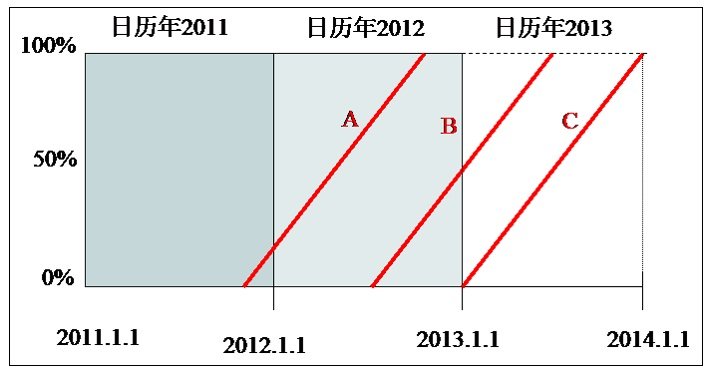
\includegraphics[width=0.6\textwidth]{Plots/calendar_year.jpg}
		\caption{按日历年汇总承保风险单位数}
	\end{figure}
\end{frame}
\begin{frame}{承保风险单位数}
	\begin{itemize}
	\item 保单A的承保日期在2011年, 保单B的承保日期在2012年, 而保单C的承保日期在2013年, 所以这三年各有一个承保风险单位数.
	
	\item 假设保单B在2013年4月1日退保, 此时该保单的期限已经完成了75\%, 剩余25\%没有完成. 在这种情况下,保单B在2012日历年的承保风险单位数仍然等于\green{1}, 但在2013日历年的承保风险单位数应该为负值, 即为\green{-0.25}.
	\end{itemize}
\end{frame}
\begin{frame}{到期风险单位数}
	原则: 看保单在该日历年度\green{有效时间}的比例. 日历年度的汇总数据在\green{当年结束}便可以得到.
	\begin{figure}
		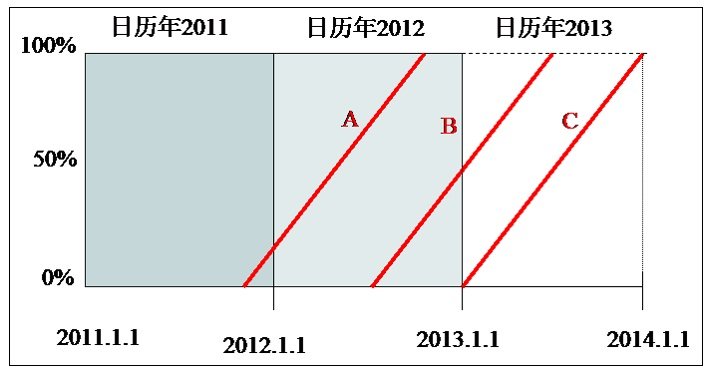
\includegraphics[width=0.6\textwidth]{Plots/calendar_year.jpg}
		\caption{按日历年度汇总到期风险单位数}
	\end{figure}
	2011: 0.25(A)\\
	2012: 0.75(A)+0.5(B)\\
	2013: 0.5(B)+1(C)
\end{frame}

\subsection{按保单年度汇总}
\begin{frame}{承保风险单位数}
	原则: 看生效日在哪个保单年. 保单年度的汇总数据在当年结束还无法得到. 保单年度的汇总数据\green{必须等到该年承保的保单都过期才能得到}. 为此引入了\red{评估日期}.
		\begin{figure}
			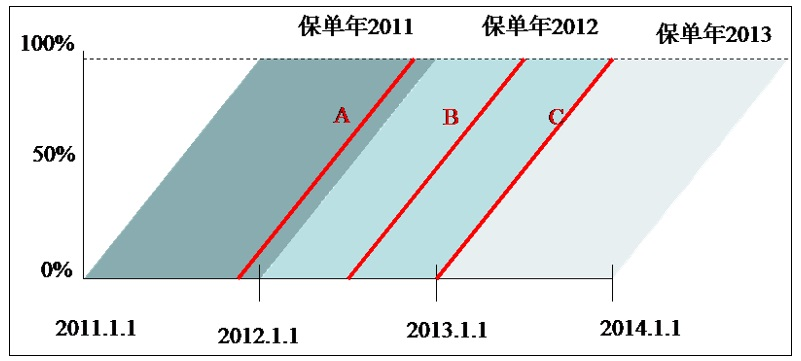
\includegraphics[width=0.6\textwidth]{Plots/policy_year.jpg}
			\caption{按保单年度汇总承保风险单位数}
		\end{figure}
		假设保单B在2013年4月1日退保. 截止到2012年12月31日, 它在2012保单年的承保风险单位数为\green{1}。截止到2013年4月2日, 它在2012保单年的承保风险单位数为\green{0.75}。
\end{frame}
\begin{frame}{到期风险单位数}
	原则: 在\red{保单年度}结束后, 按保单年度汇总的\green{到期风险单位数}等于按保单年度汇总的\green{承保风险单位数}.
		\begin{figure}
				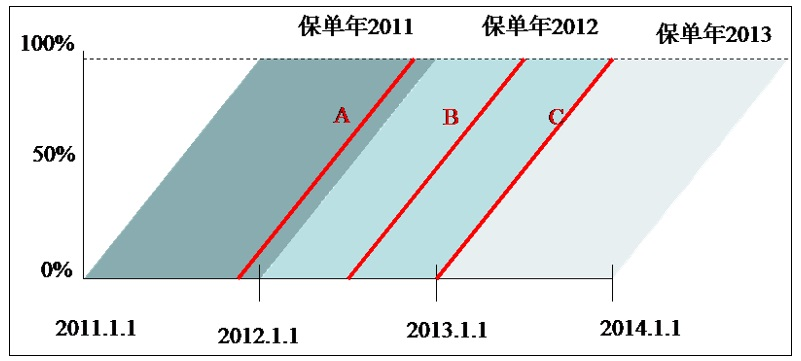
\includegraphics[width=0.7\textwidth]{Plots/policy_year.jpg}
				\caption{按保单年度汇总到期风险单位数}
			\end{figure}
对于一年期保单, 如果从保单年度的起始点计算, \green{2年}以后, 保单年度才能结束.
\end{frame}
\subsection{等水平已赚保费}
\begin{frame}
\begin{itemize}
\item Why: 若经验期费率发生变化, 需要将以前的保费调整到当前的费率水平. 注意: 赔款也会调整到当前的水平.
\item 精确方法: 将每一份保单的费率都调整到当前的费率水平.
\item \red{平行四边形近似法}: 假设\red{风险均匀分布}, 根据简单的几何关系将\green{各日历年的已赚保费}调整到当前费率水平.
\end{itemize}
\end{frame}
\begin{frame}{平行四边形近似法}
	\begin{enumerate}
		\item 确定经验期的费率变化, 根据费率变化的时间, 将保单分为不同的费率水平组 (rate level group).
		\item 计算各费率水平组的累积费率水平因子(cumulative rate level index).
		\item 计算各日历年的加权累积费率水平因子(weighted average cumulative rate level index).
		\item 计算各日历年的等水平因子(on-level factor).
		\item 计算各日历年的等水平已赚保费(on-level earned premium).
	\end{enumerate}
\end{frame}
\begin{frame}{平行四边形近似法: 例}
	\begin{figure}
		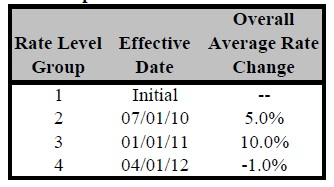
\includegraphics[width=0.4\textwidth]{Plots/on_level_1.jpg}\\
		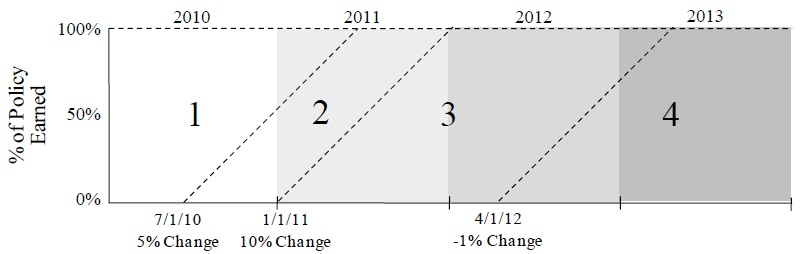
\includegraphics[width=1\textwidth]{Plots/on_level_2.jpg}

		\caption{第一步:确定费率水平组}
					\label{on_level}
		\end{figure}
\end{frame}
\begin{frame}{平行四边形近似法: 例}
	\begin{figure}
		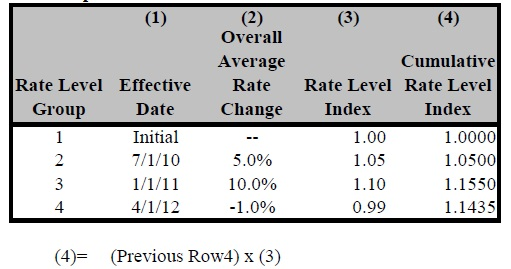
\includegraphics[width=0.6\textwidth]{Plots/on_level_4.jpg}
		\caption{第二步: 各费率水平组的累积费率水平因子}
	\end{figure}
	
\end{frame}

\begin{frame}{平行四边形近似法: 例}
	\begin{figure}
		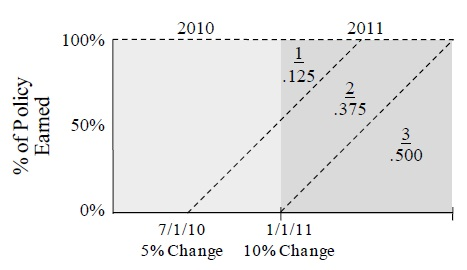
\includegraphics[width=0.6\textwidth]{Plots/on_level_3.jpg}
		\caption{第三步: 各费率水平组在2011年已赚保费中所占的比例.}
		\end{figure}

\end{frame}
\begin{frame}{平行四边形近似法: 例}
	以2011为例:
	\begin{itemize}
		\item 第三步: 2011年的加权累积费率水平因子 $1.0963=1.000\times 0.125 + 1.0500\times 0.375+ 1.1550\times0.500$ 
		\item 第四步: 2011年的等水平因子=$\frac{1.1435}{1.0963}$
		\item 第五步: 2011年等水平已赚保费=2011年已赚保费$\times$1.0431
	\end{itemize}
\end{frame}
\subsection{保费趋势的调整}
\begin{frame}
	\begin{itemize}
		\item 严格地说是\blue{平均保费水平}趋势的调整. 
		\item 等水平已赚保费是把经验期已赚保费调整到\green{当前费率}, 趋势调整是把等水平已赚保费调整到\green{未来的平均保费水平}.
		\item 平均保费水平的变化可能由以下因素引起:
		\begin{enumerate}
			\item 风险基础的膨胀: 如工伤保险, 工资不断提高.
			\item 某些重要费率因子的变化: 如车损险, 汽车价格不断上升.
			\item 保单组合中, 高费率保单的比例持续增加: 如年轻驾驶员比例持续增加.
		\end{enumerate}
	\end{itemize}
\end{frame}
\begin{frame}
	\begin{figure}
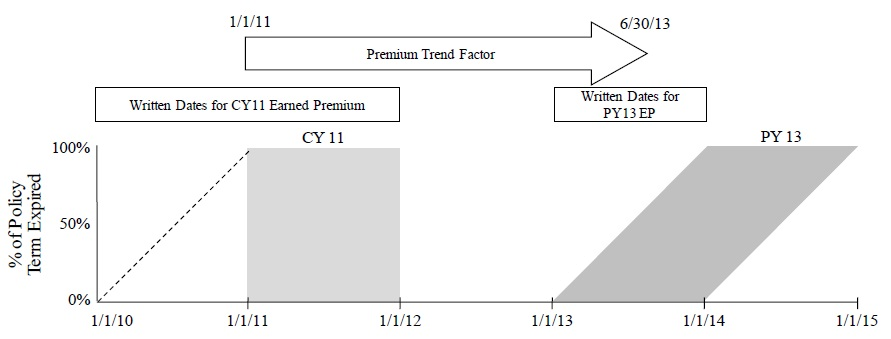
\includegraphics[width=0.8\textwidth]{Plots/Premium_trend_1.jpg}
\caption{经验期已赚保费的趋势期限.}
	\end{figure}
\end{frame}

\section{赔款数据的汇总和调整}
\begin{frame}
	\begin{itemize}
		\item 索赔数据库中的日期信息有: 生效日, 事故发生日期, 报案日期, 赔款日期.
		\item 可分别按以上的日期信息对索赔次数, 已付赔款, 已报案赔款等进行汇总.

	\end{itemize}
\end{frame}
\begin{frame}{}
例(续): 下面以表2, 3, 4的汇总表(表6)为例说明
{\tiny \begin{table}[]
		\centering
		\caption{保单ABC索赔123}
		\label{my-label}
		\begin{tabular}{ccccccccccc}
			\hline
			保单 & 索赔 & 事故        & 报案        & 交易        & 索赔   & 已付   & 个案    & AL& 残值和 \\
			编码 & 编码 & 日期        & 日期        & 日期        & 状态   & 赔款   & 准备金   &AE                       & 追偿款 \\ \hline
			A  & 1  & 2011.1.10 & 2011.1.15 & 2011.1.15 & 未结  & 0    & 10000 & 0                     & 0   \\
			A  & 1  & 2011.1.10 & 2011.1.15 & 2011.3.1  & 未结 & 1000 & 9000  & 0                     & 0   \\
			A  & 1  & 2011.1.10 & 2011.1.15 & 2011.5.1  & 已结 & 9000 & 0     & 0                     & 0   \\ \hline
			B  & 2  & 2011.10.1 & 2011.10.15 & 2011.10.15 & 未结 & 0     & 18000 & 0                     & 0    \\
			B  & 2  & 2011.10.1 & 2011.10.15 & 2011.12.15 & 未结  & 2000  & 17000 & 0                     & 0    \\
			B  & 2  & 2011.10.1 & 2011.10.15 & 2012.3.1   & 未结  & 7000  & 15000 & 0                     & 0    \\
			B  & 2  & 2011.10.1 & 2011.10.15 & 2013.3.1   & 已结 & 15000 & 0     & 0                     & 1000 \\ \hline
			C  & 3  & 2012.2.1 & 2012.2.15 & 2012.2.15 & 未结  & 0  & 15000 & 0                     & 0   \\
			C  & 3  & 2012.2.1 & 2012.2.15 & 2012.12.1 & 已结 & 0  & 0     & 1000                  & 0   \\ \hline
		\end{tabular}
	\end{table}	}
\end{frame}

\subsection{按日历年度汇总}
\begin{frame}{按交易日期计算各索赔的贡献}
	\red{日历年已报案赔款=已付赔款+个案准备金的变化\\=已付赔款+年末个案准备金-年初个案准备金}
\begin{itemize}
\item[A:]2011年(日历年)的已付赔款为10000, 个案准备金变化为0, 已报案赔款为10000. 
\item[B:]2011年(日历年)的已付赔款为2000, 个案准备金变化为17000, 已报案赔款为\green{19000}.\\
 2012年(日历年)的已付赔款为7000, 个案准备金变化为-2000, 已报案赔款为\green{5000}. \\
 2013年(日历年)的已付赔款为15000, 个案准备金变化为-15000, 已报案赔款为\green{0}.
\item[C:]2012年(日历年)已付赔款为0, 个案准备金变化为0, 已报案赔款为0.

\end{itemize}
\end{frame}
\begin{frame}{汇总所有索赔的贡献}
	\begin{itemize}
		\item[2011年:]已付赔款为10000(A)+2000(B). 已报案赔款为10000(A)+19000(B). 
		\item[2012年:]已付赔款为7000(B). 已报案赔款为5000(B).\\
		\item[2013年:]已付赔款为15000(B). 已报案赔款为0(B).
	\end{itemize}
\end{frame}
\subsection{{按事故年度汇总}}
\begin{frame}{按事故发生日期计算各索赔的贡献}
	\red{事故年已报案赔款=已付赔款+截止到评估日期的个案准备金}\\
	注: 事故年的已报案赔款受\blue{评估日期}的影响.
	
	~
	
	保单AB对2011事故年有贡献, 保单C对2012事故年有贡献. 以B为例: 
	\begin{itemize}
		\item 截止到\green{2011年末}, 2011年(\green{事故年})的已付赔款为2000, 个案准备金为17000, 已报案赔款为19000. 
		\item 截止到\green{2012年末}, 2011年(\green{事故年})的已付赔款为9000, 个案准备金为15000, 已报案赔款为24000. 
		\item 截止到\green{2013年末}, 2011年(\green{事故年})的已付赔款为24000, 个案准备金为0, 已报案赔款为24000.	此时案件已结案, 24000为最终赔款.
	\end{itemize}	
\end{frame}
\begin{frame}{汇总所有索赔的贡献}
截止到\green{2012年末}, 按事故年汇总的结果如下:
\begin{itemize}
	\item[2011年:]已付赔款为10000(A)+9000(B). 已报案赔款为10000(A)+24000(B). 
	\item[2012年:]已付赔款为0. 已报案赔款为0.\\
	\item[2013年:]已付赔款为0. 已报案赔款为0.
\end{itemize}	

~

截止到\green{2013年末}, 按事故年汇总的结果如下:
\begin{itemize}
	\item[2011年:]已付赔款为10000(A)+24000(B). 已报案赔款为10000(A)+24000(B). 
	\item[2012年:]已付赔款为0. 已报案赔款为0.\\
	\item[2013年:]已付赔款为0. 已报案赔款为0.
\end{itemize}
\end{frame}

\subsection{其它汇总方法}
\begin{frame}
	\begin{itemize}
		\item 按保单年度汇总: 即按生效日期汇总.
		\item 按报案年度汇总: 即按报案日期汇总.
	\end{itemize}
	注: 以上这两种方式汇总的结果受\green{评估日期}的影响.
\end{frame}
\subsection{最终赔款}
\begin{frame}
	计算最终赔款常用的方法为: \red{损失进展法(链梯法, chain-ladder)}. 后面, 在准备金评估模型中, 还会涉及到其它方法.
	\begin{enumerate}
		\item 按事故发生日期和进展日期(评估日期)汇编\red{流量三角形数据(run-off triangle data)}. 如\blue{累积已报案赔款(reported claims, incurred claims)或累积已付赔款(paid claims)}.
		\item 计算历史\red{进展因子(age-to-age factor)}.
		\item 计算历史进展因子的平均值(几何平均, 算术平均等).
		\item 选取未来进展因子.
		\item 选取\red{尾部因子(tail factor)}.
		\item 计算\red{累积进展因子(cumulative development factor).}
		\item 计算\red{最终赔款(ultimate claims)}.
	\end{enumerate}
\end{frame}
\begin{frame}{例-已报案赔款流量三角形}
	\begin{figure}
		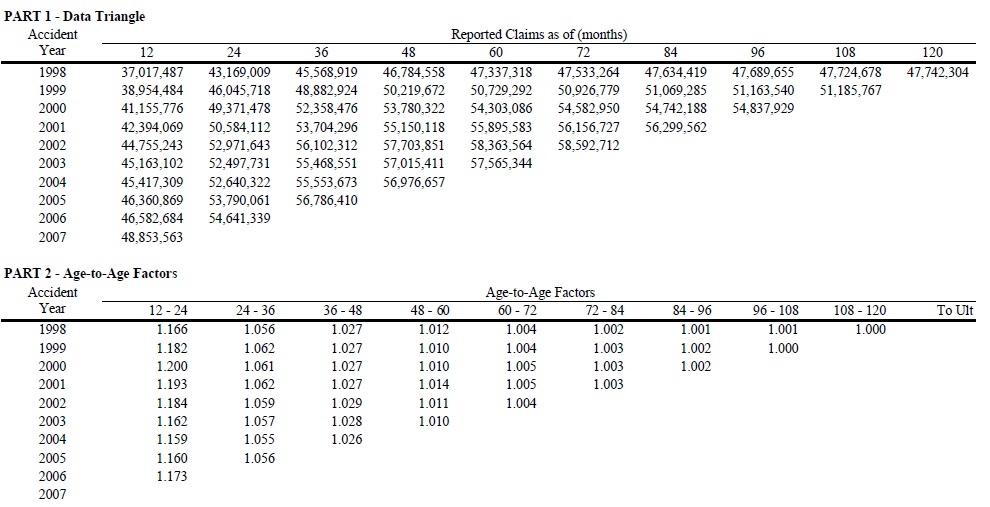
\includegraphics[width=1\textwidth]{Plots/CL1.jpg}
		\caption{汇编流量三角形, 计算进展因子}
	\end{figure}
\end{frame}
\begin{frame}{例-已报案赔款流量三角形}
	\begin{figure}
		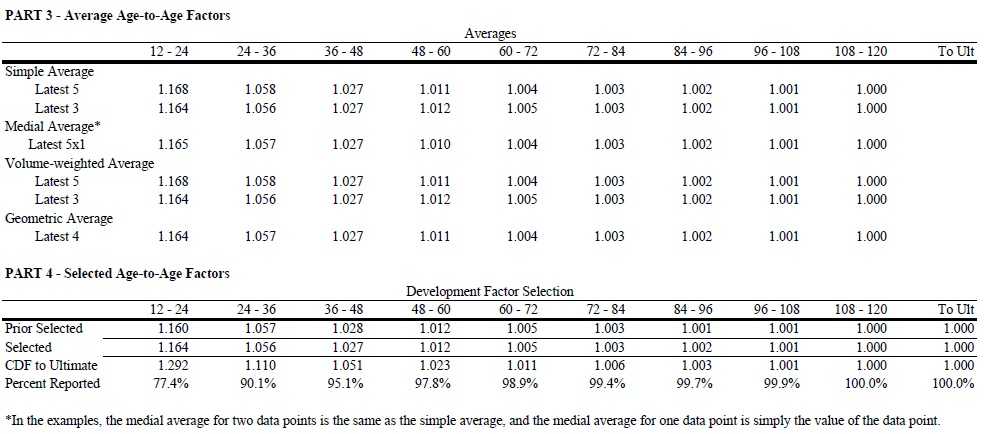
\includegraphics[width=1\textwidth]{Plots/CL2.jpg}
		\caption{计算进展因子的均值, 选取未来进展因子和尾部因子, 计算累积进展因子(CDF)}
	\end{figure}
\end{frame}
\begin{frame}{例-已付赔款流量三角形}
	\begin{figure}
		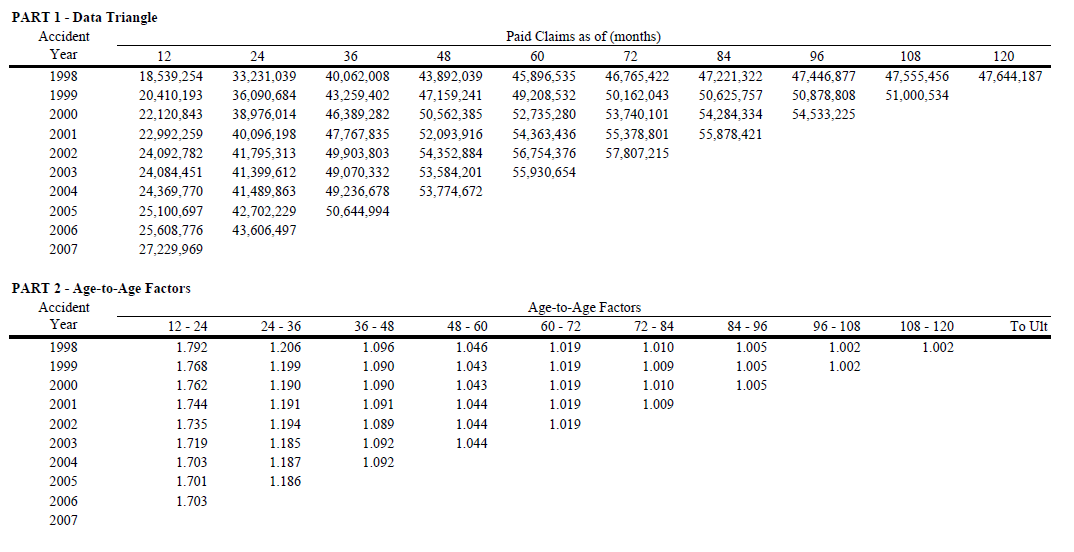
\includegraphics[width=1\textwidth]{Plots/CL3.jpg}
		\caption{汇编流量三角形, 计算进展因子}
	\end{figure}
\end{frame}
\begin{frame}{例-已付赔款流量三角形}
	\begin{figure}
		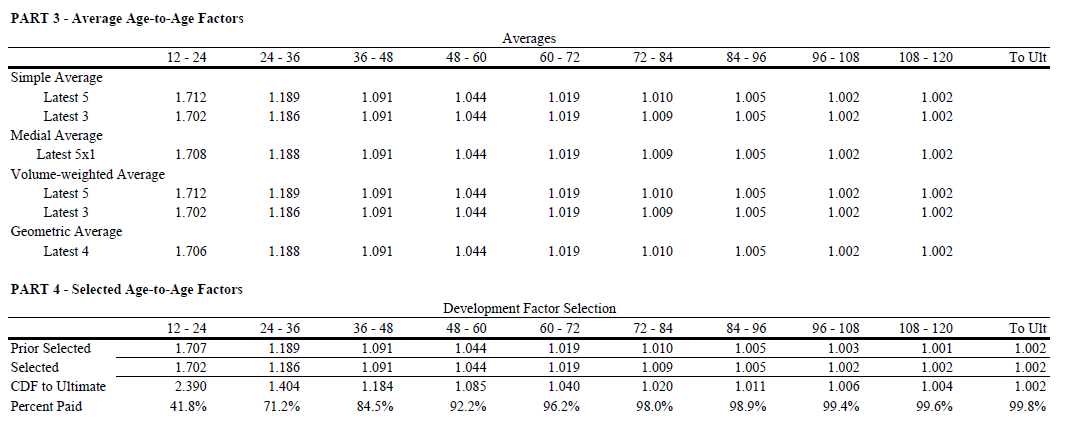
\includegraphics[width=1\textwidth]{Plots/CL4.jpg}
		\caption{计算进展因子的均值, 选取未来进展因子和尾部因子, 计算累积进展因子(CDF)}
	\end{figure}
\end{frame}
\begin{frame}{例-已报案和已付结果对比}
	\begin{figure}
		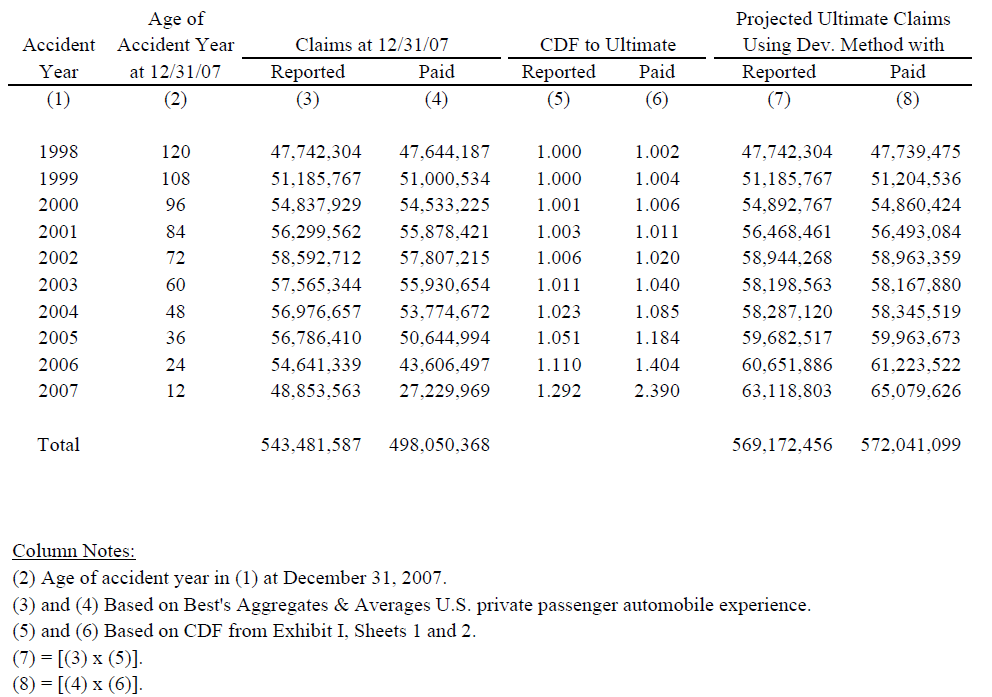
\includegraphics[width=0.8\textwidth]{Plots/CL5.jpg}
		\caption{计算最终赔款}
	\end{figure}
\end{frame}

\subsection{赔款趋势的调整}
\begin{frame}
\begin{itemize}
	\item 最终赔款从经验期到新费率应用期的变化趋势.
	\item 通常, 需要分别考虑索赔频率和索赔金额的变化趋势
	\item 引起赔款变化的因素有:
	\begin{itemize}
		\item 通货膨胀: 医疗费用上升.
		\item 安全技术的发展: 汽车ABS, 安全气囊.
		\item 业务分布的改变: 风险高的保单比例增多
		\item 非经济因素: 人们的索赔意识, 法律意识.
	\end{itemize}
\end{itemize}
\end{frame}
\begin{frame}
	\begin{figure}
		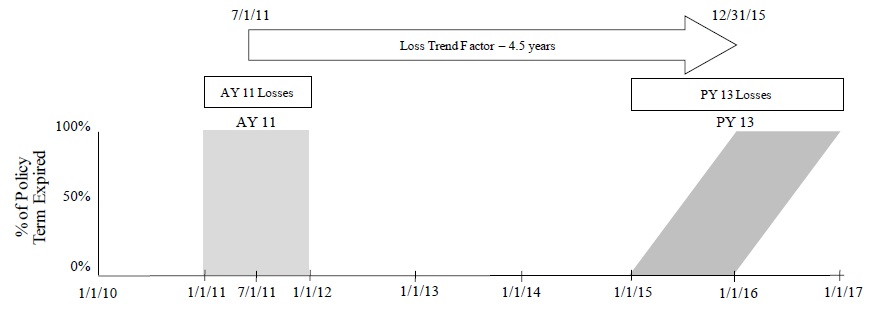
\includegraphics[width=0.8\textwidth]{Plots/Loss_trend_1.jpg}\\
		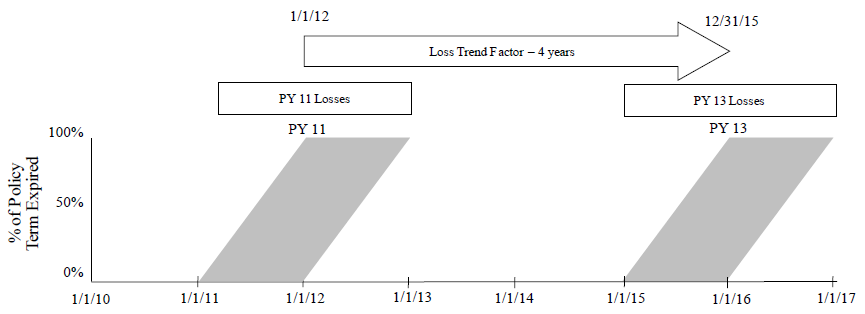
\includegraphics[width=0.8\textwidth]{Plots/Loss_trend_2.jpg}
		\caption{按事故年和保单年汇总的赔款, 其各自的趋势期限}
	\end{figure}
\end{frame}
\section{费用数据的汇总}
\begin{frame}
	\begin{itemize}
		\item 直接理赔费用: 常常和赔款合并处理.
		\item 间接理赔费用: 按照日历年度汇总, 经常表示为赔款的百分比.
		\item 承保费用: 按照日历年度汇总. 分为固定费用和变动费用, 其中变动费用经常表示为保费的百分比.
	\end{itemize}
\end{frame}

\section*{}
\begin{frame}
\begin{enumerate}
	\item 阅读教材3.2-3.3. 特别注意表3-6(赔款的汇总方法), 例3-1(平行四边形法), 表3-9(链梯法), 图3-8(保费趋势期限). 
	\item 自测课后练习题.
	\item 下载文中保单数据库和索赔数据库.\footnote{后续作业会继续使用这两个数据, 现在需要熟悉如何导入数据并做初步分析.} 
	\item 在R中安装``data.table''包, 使用fread(``ubi\_policydata.txt'') 和 fread(``ubi\_claimdata.txt'')读入数据; 检查幻灯片所列出的字段及其描述.
	
\end{enumerate}

\end{frame}
\end{document}